%-------------------------------------------------------------------------------
\section{Motivation}\label{motivation}
%-------------------------------------------------------------------------------

We now explore in further detail the benefits that serverless has to offer and
the current state of the world.

\subsection{Benefits of serverless}

The main attraction of serverless for developers is, in an idealized world, the
characteristic of only paying for what you use while having a whole datacenter
available to you. This is especially attractive to developers of applications
where the amount of resources that they need varies significantly over time, or
is generally small and very spread out, so that buying their own machines or
renting a fixed amount of server space is bad for the developer because it is
expensive if provisioned for peak usage and has poor performance if not, and bad
for the provider becuase it leads to low utilization.

A central example to this paper is that of a web server. Its traffic patterns
make it a great candidate for running entirely as serverless functions: it is
event-based, its load is bursty and unpredictable, and a request's resource
requirements can vary greatly depending on which user invoked it.


A back of the envelope calculation shows that for web servers with small load,
lambda functions as they stand today are cheaper: for a low-traffic website,
with approx 50K requests per day, a memory footprint of < 128 MB, and 200ms of
execution, running that on AWS lambda adds up to \$1.58 per month. On the other
hand, the cheapest EC2 instance costs just over \$3 per month. Of course, as the
number of requests goes up, the price for lambdas scales linearly, whereas
running an EC2 instance on full load becomes comparably cheap. There are pretty
extensive simulations that others have done that show the tradeoff points for
different types of workloads~\cite{econ-of-serverless,trek10-blog}. The provider
also loses if developers use EC2 instances for small workloads, since they are
faced with low utilization as a result.

Serverless also may outperform reservation systems for workloads that are very
bursty: starting a new lambda execution environment is much faster than starting
a new container or EC2 instance, which can take multiple
minutes~\cite{ec2-autoscaling}.


\subsection{State of the world}


\begin{figure}[t!]
    \centering
      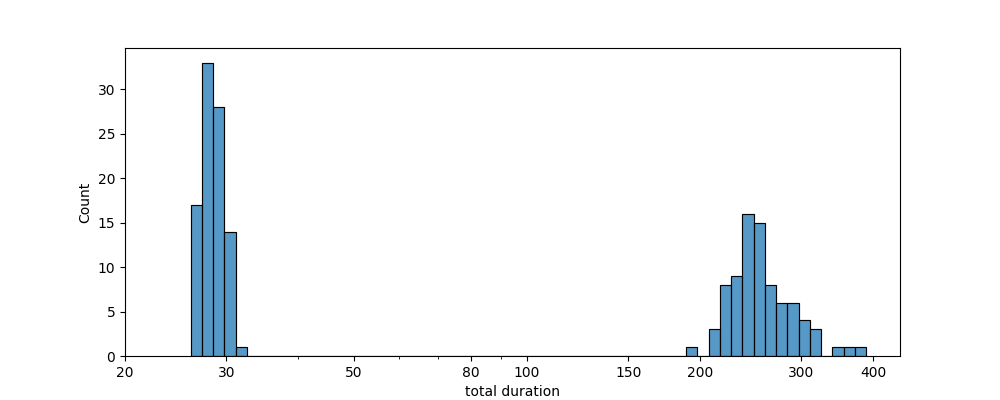
\includegraphics[width=8.5cm]{img/lambda_total_durations.png}
      \caption{ distribution of end to end duration times. The x axis is log scale }
    \label{fig:lambda-total-durations}
\end{figure}

However, only few web servers run entirely on serverless offerings today. There
are many reasons that developers choose not to use serverless, despite their
workloads being well-suited for the serverless
environment~\cite{not-lambda-blog,reddit-serverless2}. Popular complaints
include provider lock in, lack of insight for debugging and telemetry, and
variable runtimes.


\Sys{} focuses on the technial challenge of variable runtimes. In order to
better understand the where the variation comes from, we run an experiment with
a simple lambda function that sleeps for 20ms and then returns. We use AWS
Xray~\cite{aws-xray} to measure its latency, with incovations spaced randomly
between 0 and 10 minutes. The results are in
Figure~\ref{fig:lambda-total-durations}. The times on the left side of the graph
are clearly the execution times from warm start, which remain somewhat stable.
The reason for this is that AWS is able to simply route the new request to the
machine with the existing container on it. We verify that this is indeed what is
happening by changing the function to include reading and then writing to an
environment variable, and find that for invocations with warm start when we read
the variable it was already set by a previous invocation.

The right grouping in the graph is then the invocations that hit cold starts,
whose overall latencies vary between 200 and 400ms, meaning that when a request
encounters cold start, the variance in observed latency goes up a lot.

\begin{figure}[t!]
  \centering
    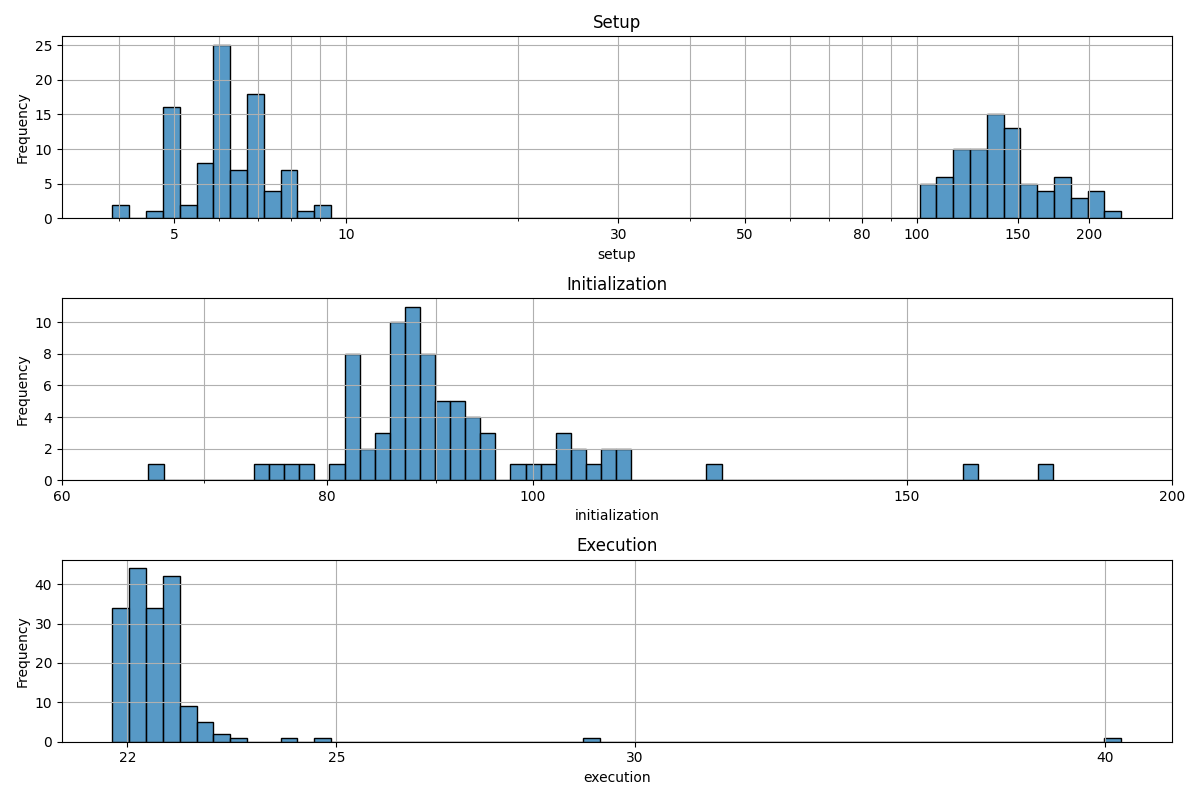
\includegraphics[width=8.5cm]{img/lambda_duration_breakdown.png}
    \caption{ Breakdown of variation in duration times. X axes are all log scale }
  \label{fig:lambda-durations-breakdown}
\end{figure}

In order to better understand where that variability comes from, we look into a
breakdown of the latencies. We are able to break down the total duration into
three components: \textit{setup}, which includes placing the function and
creating the container; \textit{initialization}, which is any code that runs
before the function does, for example initializing the runtime, and any python
modules the function uses; and \textit{execution}, actually executing the
functions code. Xray gives us only the latter two values explicitly, we
calculate the setup time by looking at the total duration and subtracting the
initalization and execution times. 

We can see the resulting distributions in
Figure~\ref{fig:lambda-durations-breakdown}. The most stable component of the
duration is unremarkably the execution time, although with some outliers. The
initialization time has a fair amount of variance, although there are no
discernable groupings. The strongest variability, unsurprisingly, comes from the
setup portion. Here we can see the two groupings clearly: one on the right that
includes starting up the container, and one on the left that doesn't. The range
is larger on the right ($\sim$150ms) than it is on the left ($\sim$8ms).

We can conclude that there is already a small variation in warm start setting,
where AWS doesn't even need to place a new container; and clear is also that
sometimes AWS is able to get the cold start container up and running in just
over 100ms, and sometimes it takes as much as $\sim$250ms. Where exactly the
latency here comes from is impossible to know without futher insight into the
system.

In order to further understand the dynamics of when AWS uses existing
containers, we build an experiemnt to understad whether AWS will use any
container of the correct runtime (within the same tenant). We run the following
experiment: two different functions, foo and bar, that both use the exactly same
runtime (the AWS Python 3.13 environment), and we use the same trick as above of
reading and then setting an environment variable to a function-specific value.
We first run foo once, and then immediately fire off 100 parallel invocations of
bar. Even though many of the bar invocations experience cold start, those that
have warm start are reusing containers from already completed bar invocations;
none of them use the container created by foo. 

It might seem desirable to be able to use a different functions warm container,
but that would require AWS being able to know which function should have
priority over the other in order to know which to preempt vs to let run to
completion in the case that invocations of two different functions are competing
for the same container. Instead, AWS offers two different ways for developers to
influence their functions' scaling: provisioned and reserved
concurrency\cite{aws-scaling}. Provisioned concurrency specifies a number of
instances to keep warm for a given function, and reserved concurrency ensures
that a fixed amount of the possible concurrency reserved for it. This interface,
although effective at avoiding cold starts, moves away from the serverless
approach of on-demand resources and paying for what you use; instead requiring
developers to estimate their future needs and pay up front, and providers to set
aside those potentisally idle resources.



